

This part of the development process aims to add two new features to the output application of the previous step. This process is divided into two subprocesses. Both of them aims to add a single new feature.

\paragraph{The Add todo Feature - }
\label{par:add_todo_feature}
The first subproces adds the possibility to create new todos. It utilizes the FloatingActionButton widget, already present in the bottom right corner of the application, to push a new page called: AddTodoPage. In the AddTodoPage is possible to compile two TextField widgets and utilize a TextButton widget to return to the HomePage creating the new todo.
 

\begin{figure}[H]
    \centering
    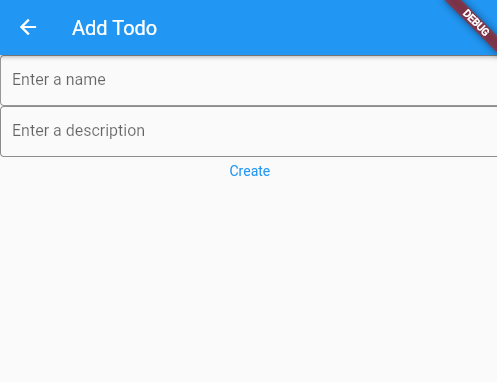
\includegraphics[width=0.5\textwidth]{Images/shot_runtime_todoapp_addpage.png}
    \caption{Shows the AddTodoPage UI}
    \label{fig:add_todo_page_tree_structure}
\end{figure}
\paragraph{The Update feature - }
\label{par:update_todo_feature}
The second subproces aims to add the possibility to update existing todos. Tapping on a specific TodoItem allow to navigate to a new page : the UpdateTodoPage. In the UpdateTodoPage is possible to compile two TextFields widgets and use a TextButton widget to return to the HomePage modifing the corresponding todo.

\begin{figure}[H]
    \centering
    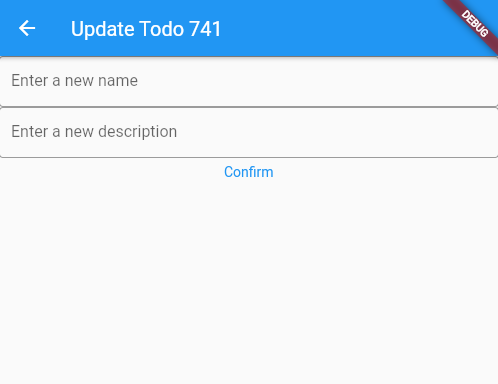
\includegraphics[width=0.5\textwidth]{Images/shot_runtime_todoapp_updatepage.png}
    \caption{Shows the UpdateTodoPage UI for the todo with id 741}
    \label{fig:add_todo_page_tree_structure}
\end{figure}